%------------------------------------------------------------------------------

\newpage
\pagestyle{empty}

\subsubsection{About the Author}


\begin{wrapfigure}{r}{0.43\textwidth}
\vspace{-35px}
\begin{center}
 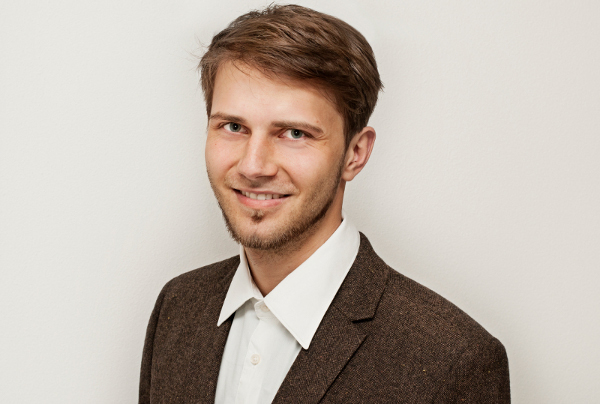
\includegraphics[width=0.42\textwidth]{Cover/TobiasHolzmann.jpg}
\end{center}
\vspace{-30px}
\end{wrapfigure}
This book is a present to the \OF community written by Tobias Holzmann.
Since 2009, Tobias is working in the field of numerical simulations. During his
studies at the Fachhochschule Augsburg, he decided to write his Bachelor thesis
in the field of heat transfer using numerical tools such as \OF including
validations against measurements.

During his Master's study, he focused on topics related to numerical simulations.
During that time, he started to compare the quantitative results of different
phenomena using ANSYS\textregistered~CFX and \OF. Finally, he finished his
Masters' study investigation in biomass combustion modeling using the flamelet
model and \OF. After that, he started to publish his knowledge in the field of
numerical simulations and \OF on his private website to support the \OF
community people. In 2014, Tobias started his Ph.D. at
the Montanuniversität Leoben. There, he investigated local heat treatments
of aluminum alloys. The main topics were thermal stress analysis, material
kinetics related to heterogeneous local heat treatment in 3D, and optimization.

After Tobias started his Ph.D. in 2014, he decided to investigate more into the
field of numerical mathematics, matrix algebra, derivations, and advanced
c++ programming. During his Ph.D., Tobias published different material regarding
\OF, training cases, and publications. In 2017 he became an
official contributor to the OpenFOAM Foundation branch, mainly in the
conjugated heat transfer, thermal comfort analysis, and several features and
extensions.

Tobias is a moderator in the German \OF forum, namely cad.de as well
as in the well-known cfd-online.com forum. All his projects, developments, and
investigations are published under the GPL v3 on his website
\url{https://Holzmann-cfd.com}. Tobias hopes that his material and effort helps
people all over the world.
\\~\\
Keep Foaming...\\
Dr. mont. Tobias Holzmann


%------------------------------------------------------------------------------
